% Chapter 5: Security Mechanisms (Guardrails)

\begin{frame}{Chapter 5: Security Mechanisms (Guardrails)}
    \begin{center}
        \Large{\textbf{Chapter 5}}\\
        \vspace{0.5em}
        \huge{\textbf{Security Mechanisms}}\\
        \huge{\textbf{(Guardrails)}}\\
        \vspace{0.5em}
        \large{Ensuring Safety in Medical AI Systems}
    \end{center}
    
    \vspace{0.5em}
    
    \textbf{Medical Domain Challenges:}
    \begin{itemize}
        \item \textbf{Unauthorized diagnosis:} System must not replace doctors
        \item \textbf{Drug prescriptions:} No specific treatment recommendations
        \item \textbf{PHI protection:} HIPAA compliance requirements
        \item \textbf{Emergency situations:} Proper escalation procedures
        \item \textbf{Drug interactions:} Preventing dangerous advice
    \end{itemize}
\end{frame}

\begin{frame}{Guardrails Architecture and Input Policies}
	\begin{columns}[T]
		\column{0.5\textwidth}
		\textbf{Multi-layer Architecture:}
		\begin{center}
			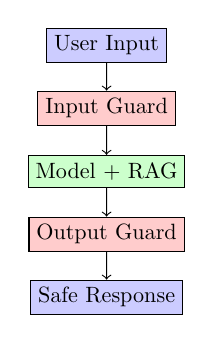
\begin{tikzpicture}[node distance=1cm, scale=0.8, transform shape]
				\node[rectangle,draw,fill=blue!20] (input) {User Input};
				\node[rectangle,draw,fill=red!20,below of=input] (inputguard) {Input Guard};
				\node[rectangle,draw,fill=green!20,below of=inputguard] (model) {Model + RAG};
				\node[rectangle,draw,fill=red!20,below of=model] (outputguard) {Output Guard};
				\node[rectangle,draw,fill=blue!20,below of=outputguard] (output) {Safe Response};
				
				\draw[->] (input) -- (inputguard);
				\draw[->] (inputguard) -- (model);
				\draw[->] (model) -- (outputguard);
				\draw[->] (outputguard) -- (output);
			\end{tikzpicture}
		\end{center}
		
		\column{0.5\textwidth}
		\textbf{Nine Input Controls:}
		\begin{enumerate}
			\footnotesize
			\item No personal diagnosis requests
			\item Protection of safety rules
			\item Emergency situation management
			\item Sensitive content filtering
			\item Abusive language prevention
			\item PHI protection
			\item Identity impersonation prevention
			\item System security
			\item Malicious code blocking
		\end{enumerate}
	\end{columns}
	
	\vspace{0.5em}
	\begin{center}
		\colorbox{red!20}{\textbf{Blocks inappropriate requests before processing}}
	\end{center}
\end{frame}


\begin{frame}{Output Policies and Technical Challenges}
    \textbf{Eight Core Output Criteria:}
    \begin{columns}[T]
        \column{0.5\textwidth}
        \begin{itemize}
            \footnotesize
            \item \textbf{Harm prevention:} No dangerous advice
            \item \textbf{Professional disclaimer:} Not doctor replacement
            \item \textbf{Treatment limitations:} No specific recommendations
            \item \textbf{Information accuracy:} No misinformation
        \end{itemize}
        
        \column{0.5\textwidth}
        \begin{itemize}
            \footnotesize
            \item \textbf{Self-diagnosis prevention:} No self-treatment
            \item \textbf{Evidence-based:} Avoid unverified claims
            \item \textbf{Appropriate tone:} Clear, empathetic
            \item \textbf{Proper referrals:} Direct to professionals
        \end{itemize}
    \end{columns}
    
    \vspace{0.5em}
    
    \textbf{Implementation Challenges:}
    \begin{itemize}
        \item Balance between safety and usability
        \item \textcolor{red}{\textbf{176\% increase in response time}} (additional 730ms)
        \item Comprehensive scenario coverage
        \item Bilingual support (Persian/English)
        \item Context detection challenges
        \item Increased computational load
    \end{itemize}
    
    \begin{center}
        \colorbox{green!20}{\textbf{Ensures safe and appropriate responses}}
    \end{center}
\end{frame}

\begin{frame}{Optimization Strategies and Summary}
    \begin{columns}[T]
        \column{0.5\textwidth}
        \textbf{Performance Optimization:}
        \begin{itemize}
            \item Lighter specialized models
            \item Parallel processing
            \item Result caching
            \item Rule-based filtering for obvious cases
        \end{itemize}
        
        \column{0.5\textwidth}
        \textbf{Accuracy Enhancement:}
        \begin{itemize}
            \item Continuous learning from feedback
            \item Threshold optimization
            \item Multi-technique combination
            \item Adaptive sensitivity
        \end{itemize}
    \end{columns}
    
    \vspace{0.5em}
    
    \textbf{Key Achievements:}
    \begin{itemize}
        \item Comprehensive medical safety framework implemented
        \item 17 total policies (9 input + 8 output)
        \item Bilingual support for Persian and English
        \item Critical protective layer for medical AI deployment
    \end{itemize}
    
    \vspace{0.5em}
    
    \textbf{Current Limitations:}
    \begin{itemize}
        \item \textcolor{red}{176\% latency increase} needs optimization
        \item Need for continuous policy updates
        \item Cultural adaptation requirements
    \end{itemize}
    
    \begin{center}
        \colorbox{highlight!20}{\textbf{Goal: Reduce latency while maintaining safety}}
    \end{center}
\end{frame}
